\documentclass[serif, aspectratio=169]{beamer}
\usepackage[T1]{fontenc} 
\usepackage{fourier}
\usepackage{hyperref}
\usepackage{latexsym,amsmath,xcolor,multicol,booktabs,calligra}
\usepackage{booktabs} % For better table formatting
\usepackage{graphicx,pstricks,listings,stackengine}
\usepackage{listings}
\usepackage{array} 
\usepackage{colortbl}

\author{Dr.Hajialiasgari}
\title{Machine Learning}
\institute{
    Tehran University \\
    Of\\
    Medical Science
}
\date{\small \today}
\usepackage{UoWstyle}

% Define custom colors and styles for listings
\definecolor{deepblue}{rgb}{0,0,0.5}
\definecolor{deepred}{RGB}{153,0,0}
\definecolor{deepgreen}{rgb}{0,0.5,0}
\definecolor{halfgray}{gray}{0.55}

\lstset{
    basicstyle=\ttfamily\small,
    keywordstyle=\bfseries\color{deepblue},
    emphstyle=\ttfamily\color{deepred},
    stringstyle=\color{deepgreen},
    numbers=left,
    numberstyle=\small\color{halfgray},
    rulesepcolor=\color{red!20!green!20!blue!20},
    frame=shadowbox,
}

\begin{document}

\begin{frame}
    \titlepage
    \vspace*{-0.6cm}
    \begin{figure}[htpb]
        \begin{center}
            \includegraphics[keepaspectratio, scale=0.05]{Tumsl-logo.png}
        \end{center}
    \end{figure}
\end{frame}

\begin{frame}    
\tableofcontents[sectionstyle=show, subsectionstyle=show/shaded/hide, subsubsectionstyle=show/shaded/hide]
\end{frame}

\section{Overview}

\begin{frame}{Parametric vs. Non-Parametric Methods in Classification}
    \textbf{1. Parametric Methods}
    \begin{itemize}
        \item \textbf{Definition}: Assume a specific form (parametric model) for the decision boundary or the data distribution.
        \item \textbf{Examples}: Logistic regression, Naive Bayes, Linear Discriminant Analysis (LDA).
        \item \textbf{Advantages}:
        \begin{itemize}
            \item Simple and computationally efficient.
            \item Easy to interpret.
            \item Work well with smaller datasets if assumptions hold.
        \end{itemize}
        \item \textbf{Disadvantages}:
        \begin{itemize}
            \item Relies heavily on the correctness of the assumed model.
            \item May perform poorly if the true relationship deviates from the assumed model.
        \end{itemize}
    \end{itemize}
\end{frame}
\begin{frame}{Parametric Vs Non-Parametric Methods in Classification}
    
    \textbf{2. Non-Parametric Methods}
    \begin{itemize}
        \item \textbf{Definition}: Do not assume any specific form for the data distribution. 
        \item \textbf{Examples}: k-Nearest Neighbors (k-NN), Decision Trees, Support Vector Machines (SVM), Random Forests.
        \item \textbf{Advantages}:
        \begin{itemize}
            \item Flexible and can model complex patterns in data.
            \item Often perform better when the relationship between input features and target is unknown or nonlinear.
        \end{itemize}
        \item \textbf{Disadvantages}:
        \begin{itemize}
            \item Higher computational cost, especially with large datasets.
            \item May overfit if not properly regularized or pruned.
        \end{itemize}
    \end{itemize}
\end{frame}

\begin{frame}{Key Differences: Parametric vs. Non-Parametric}
    \begin{table}[]
        \centering
        \begin{tabular}{|l|l|l|}
        \hline
        \textbf{Feature}         & \textbf{Parametric Methods} & \textbf{Non-Parametric Methods} \\ \hline
        \textbf{Assumptions}     & Strong (e.g., linearity)    & Minimal or none                \\ \hline
        \textbf{Flexibility}     & Limited                    & High                           \\ \hline
        \textbf{Data Requirement}& Low                        & High                           \\ \hline
        \textbf{Complexity}      & Simple                     & Complex                        \\ \hline
        \end{tabular}
    \end{table}
\end{frame}

\begin{frame}{Example Applications}
    \textbf{Parametric Methods:}
    \begin{itemize}
        \item Logistic regression for predicting a binary outcome like spam detection.
    \end{itemize}
    \textbf{Non-Parametric Methods:}
    \begin{itemize}
        \item k-NN for classifying handwritten digits.
    \end{itemize}
\end{frame}

\begin{frame}{k-Nearest Neighbors (k-NN)}
    \textbf{Overview:}
    \begin{itemize}
        \item k-Nearest Neighbors (k-NN) is a non-parametric, lazy learning algorithm.
        \item Used for both classification and regression tasks.
    \end{itemize}

    \textbf{Key Features:}
    \begin{itemize}
        \item \textbf{Non-Parametric:} Makes no assumptions about data distribution.
        \item \textbf{Lazy Learning:} No explicit training; stores data and predicts only when required.
        \item \textbf{Instance-Based:} Predictions rely on similarity between new and training data.
    \end{itemize}
\end{frame}

\begin{frame}{How k-NN Works}
    \begin{enumerate}
        \item \textbf{Calculate Distance:} Compute the distance (e.g., Euclidean) between the new data point and all training points.
        \item \textbf{Find Nearest Neighbors:} Identify the $k$ closest training points.
        \item \textbf{Vote (Classification):} Assign the class that is most common among the $k$ neighbors.
        \begin{itemize}
            \item For regression: Use the mean or weighted average of the neighbors' values.
        \end{itemize}
    \end{enumerate}

    \textbf{Choosing $k$:}
    \begin{itemize}
        \item Small $k$: Sensitive to noise and overfits.
        \item Large $k$: Robust but may underfit.
        \item Optimal $k$: Found via cross-validation.
    \end{itemize}
\end{frame}

\begin{frame}{Advantages and Disadvantages of k-NN}
    \textbf{Advantages:}
    \begin{itemize}
        \item Simple and easy to implement.
        \item No explicit training phase; quickly adapts to new data.
        \item Effective for small datasets with low dimensions.
    \end{itemize}

    \textbf{Disadvantages:}
    \begin{itemize}
        \item Computationally expensive for large datasets.
        \item Sensitive to noisy or irrelevant features.
        \item Requires careful choice of distance metric.
    \end{itemize}
\end{frame}

\begin{frame}{KNN Algorithm Visualization}
    \hspace*{\fill}
    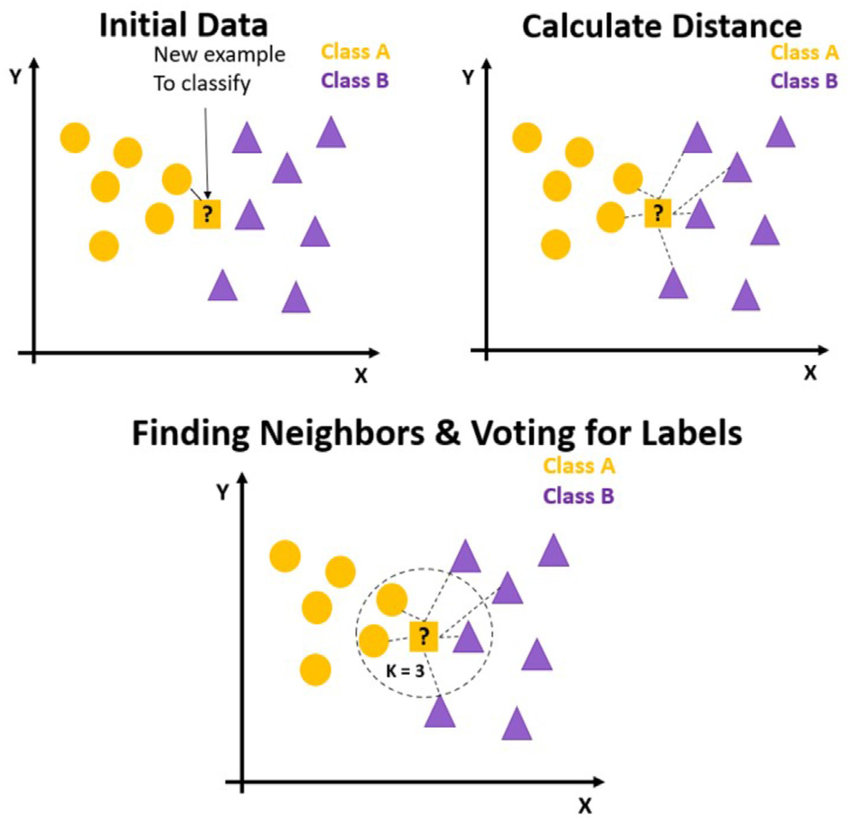
\includegraphics[width=0.45\textwidth]{An-example-of-KNN-algorithm.png}
    \hspace*{\fill}
\end{frame}


\begin{frame}{Distance Calculation in KNN}
    \textbf{Distance Calculation:}
    \begin{itemize}
        \item Euclidean Distance:
        \[
        d(x, x_i) = \sqrt{\sum_{j=1}^n (x_j - x_{ij})^2}
        \]
        \item Manhattan Distance:
        \[
        d(x, x_i) = \sum_{j=1}^n |x_j - x_{ij}|
        \]
        \item Minkowski Distance (generalized):
        \[
        d(x, x_i) = \left( \sum_{j=1}^n |x_j - x_{ij}|^p \right)^{1/p}
        \]
    \end{itemize}
\end{frame}

\begin{frame}{Predicion in KNN}
    \textbf{Prediction:}
    \begin{itemize}
        \item For Classification:
        \[
        \hat{y} = \text{argmax}_c \sum_{i \in N_k} \mathbb{I}(y_i = c)
        \]
        where \( N_k \) is the set of \( k \)-nearest neighbors and \( \mathbb{I} \) is the indicator function.
        \item For Regression:
        \[
        \hat{y} = \frac{1}{k} \sum_{i \in N_k} y_i
        \]
    \end{itemize}
\end{frame}

\begin{frame}{Effect of K}
    \hspace*{\fill}
    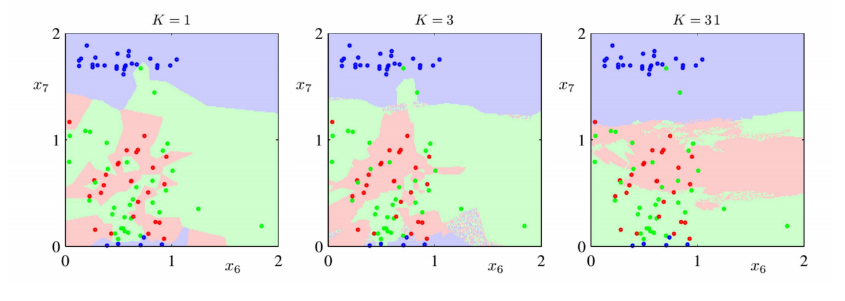
\includegraphics[width=0.75\textwidth]{fJG0H.png}
    \hspace*{\fill}
\end{frame}

\begin{frame}{Effect of k}
    \hspace*{\fill}
    \includegraphics[width=0.75\textwidth]{file.png}
    \hspace*{\fill}
\end{frame}

\begin{frame}{kNN for Regression}

    \item Although k-NN is primarily introduced for classification tasks, it can also be adapted for regression problems with some modifications. For instance, after identifying the nearest neighbors, instead of using majority voting, we can take the mean or median of the target variable values of these neighbors and use it as the predicted value.
    
\end{frame}

\begin{frame}{KNN for Linear Regression}
    \hspace*{\fill}
    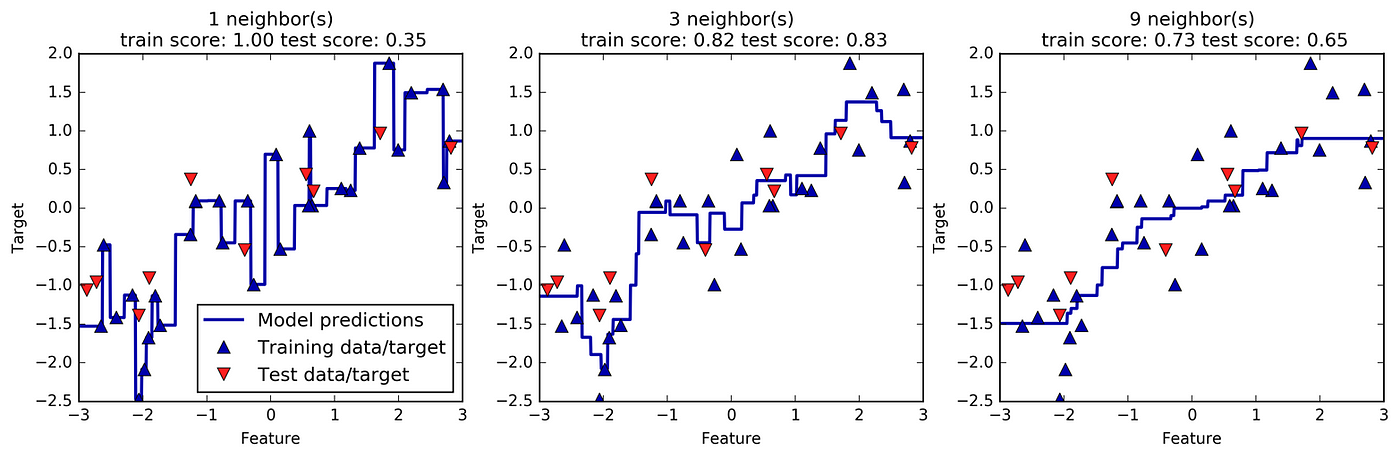
\includegraphics[width=0.75\textwidth]{KNN-for-LR.png}
    \hspace*{\fill}
\end{frame}

\section{Cross Validation}

\begin{frame}{Cross Validation}
\begin{itemize}
    \item \textbf{Purpose:} Technique for evaluating how well a model generalizes to unseen data.
    \item \textbf{How It Works:} Split data into $k$ folds; train on $k-1$ folds and validate on the remaining fold.
    \item \textbf{Repeat Process:} Repeat $k$ times, rotating the test fold each time. Average of all scores is the final score of the model.
    \item Cross-validation reduces overfitting and provides a more reliable estimation of model performance.
    \item \textbf{Note:} The model must be retrained at each iteration to avoid reusing a model that has already seen the test data, ensuring unbiased evaluation.
\end{itemize}
\end{frame}


\begin{frame}{K-Fold Cross Validation}
    \hspace*{\fill}
    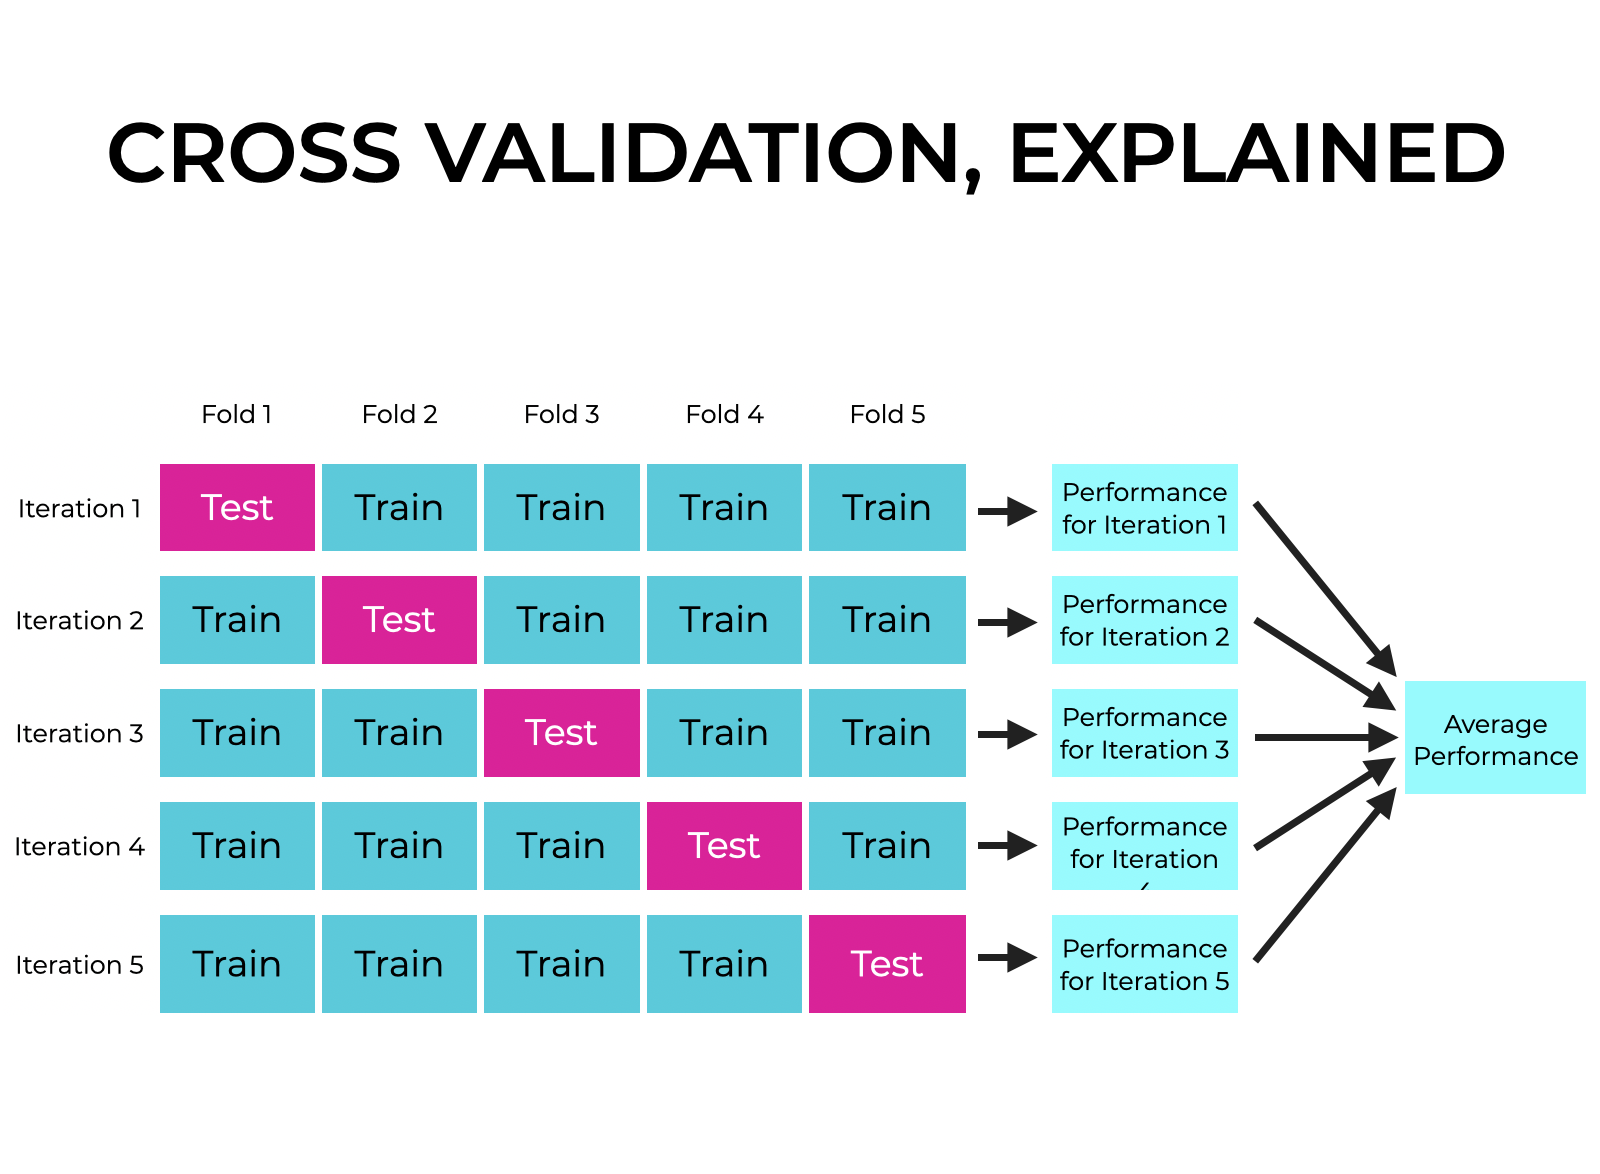
\includegraphics[width=0.45\textwidth]{cross-validation.png}
    \hspace*{\fill}
\end{frame}

\begin{frame}{Leave-One-Out Cross-Validation (LOOCV)}
\begin{itemize}
    \item \textbf{How It Works:} Uses a single data point as the validation set ($k = 1$) and the rest as the training set. Repeat for all data points.
    \item \textbf{Properties:}
    \begin{itemize}
        \item No Data Wastage: Every data point is used for both training and validation.
        \item High Variance, Low Bias.
        \item Computationally Expensive: Requires training the model $N$ times for $N$ data points, making it slow for large datasets.
        \item Best for small datasets.
    \end{itemize}
\end{itemize}
\end{frame}


\begin{frame}
    \begin{center}
        {\Huge\ \color{red}For more information and code check the related notebook}
    \end{center}
\end{frame}


\begin{frame}
    \begin{center}
        {\Huge\ End of Classification}
    \end{center}
\end{frame}

\end{document}

